\documentclass{article}

\usepackage{amssymb,amsmath,amsfonts,amsthm,stmaryrd,fancyhdr,graphicx,epic,eepic,pifont}
\usepackage{bbding}

%\usepackage{showkeys} %%% This package will show you your labels
                       %%% and should be commented out for the 
                       %%% final print out.
\usepackage{makeidx} %%% gives us our groovy index
\makeindex

%%% This sets how the enumerate command works
\renewcommand{\labelenumi}{$(\mathrm{\arabic{enumi}})$}


%%% This next bit of code defines all our theorem environments
\newtheoremstyle{SlantTheorem}{\topsep}{\topsep}%%% space between body and thm
		{\slshape}                      %%% Thm body font
		{}                              %%% Indent amount (empty = no indent)
		{\bfseries\sffamily}            %%% Thm head font
		{}                              %%% Punctuation after thm head
		{3ex}                           %%% Space after thm head
		{\thmname{#1}\thmnumber{ #2}\thmnote{ \bfseries(#3)}}%%% Thm head spec
\theoremstyle{SlantTheorem}
\newtheorem*{thm}{Theorem}
\newtheorem*{para}{Paradox}
\newtheorem*{con}{Construction}
\newtheorem*{conj}{Conjecture}
\newtheorem*{cor}{Corollary}
\newtheorem*{war}{WARNING}
\newtheorem*{eg}{Example}

\newtheoremstyle{Definition}
{\topsep}{\topsep}{}{}{\sffamily\bfseries}{}{3ex}{}
\theoremstyle{Definition}
\newtheorem*{dfn}{Definition}

\newtheoremstyle{Exercises}
{\topsep}{\topsep}{}{}{\bfseries}{}{3ex}{}
\theoremstyle{Exercises}
\newtheorem{ques}{Question}
\newtheorem*{prob}{Problem}

\usepackage{array}
\setlength{\extrarowheight}{0cm}
\newdimen\digitwidth
\settowidth\digitwidth{9}
\def~{\hspace{\digitwidth}}
\def\divrule#1#2{
\noalign{\moveright#1\digitwidth
\vbox{\hrule width#2\digitwidth}}}



%%% This bit of code gives us our nice proof environment.
\renewenvironment{proof}[1][\proofname]{\begin{trivlist}\item[\hskip \labelsep \itshape \bfseries #1{}\hspace{2ex}]}
{\qed\end{trivlist}}
%%%

%%% This set of code gives us the unnumbered footnotes
\long\def\symbolfootnote[#1]#2{\begingroup\def\thefootnote{\fnsymbol{footnote}}
\footnote[#1]{#2}\endgroup}



%%% This set of code is all of our user defined commands
\newcommand{\bysame}{\mbox{\rule{3em}{.4pt}}\,}
\newcommand{\N}{\mathbb N}
\newcommand{\Z}{\mathbb Z}
\newcommand{\R}{\mathbb R}
\newcommand{\Q}{\mathbb Q}
\newcommand{\A}{\mathbb A}
\newcommand{\C}{\mathcal C}
\newcommand{\ph}{\varphi}
\newcommand{\ep}{\varepsilon}
\newcommand{\aph}{\alpha}
\newcommand{\QM}{\begin{center}{\huge\textbf{?}}\end{center}}
\renewcommand{\le}{\leqslant}
\renewcommand{\ge}{\geqslant}
\renewcommand{\a}{\wedge}
\renewcommand{\v}{\vee}
\renewcommand{\l}{\ell}
\renewcommand{\subset}{\subseteq}
\renewcommand{\supset}{\supseteq}
\renewcommand{\emptyset}{\varnothing}
\renewcommand{\qedsymbol}{$\blacksquare$}

\newcommand{\tri}{\triangle}



\newcommand{\mat}{\mathsf}
\renewcommand{\vec}{\mathbf}


\renewcommand{\labelenumi}{$(\mathrm{\alph{enumi}})$}

\begin{document}

\section*{Cube Root of Two} %%remove * if added to notes!

!!!MISTAKE!!! USE $F_i$ instead of $\Q$. 
!!!WILL NEED A ``BUCKET OF NUMBERS'' HANDOUT TO PRECEED THIS ONE!!!

In this handout we are going to see why the cube root of two is not
construcitable with compass and straightedge alone. First let's look
at a plot of $x^3-2$:
\[
\includegraphics[width=3in]{../graphics/cube2.eps}
\]
\begin{ques} 
How many complex roots does $x^3-2$ have? How many real roots does
$x^3-2$ have?
\end{ques}

\begin{ques} Explain why every number in $\C$ can be expressed as 
\[
p + q \sqrt{n} 
\]
where $p,q\in \Q$, $n\in \N$, with $\sqrt{n}\notin\Q$.
\end{ques}

We are going to suppose that $a^3 - 2= 0$. Could $a\in\C$? If so, by
our previous work we would have that 
\[
a = p + q\sqrt{n}
\]
where $p,q\in \Q$, $n\in \N$, with $\sqrt{n}\notin\Q$.

\begin{ques}\label{Q:s} Use the Binomial Theorem to expand $a^3 -2$:
\[
(p + q\sqrt{n})^3 -2
\]
\end{ques}

\begin{ques} Collect like terms to write
\[
(p + q\sqrt{n})^3 -2
\]
as 
\[
P + Q \sqrt{n}
\]
\end{ques}

\begin{ques} A little bird told me that at this point we must conclude that:
\[
P + Q \sqrt{n} = 0
\]
Why is that again?
\end{ques}

\begin{ques}\label{Q:f} If $P + Q \sqrt{n} = 0$ and $Q \ne 0$, then we can write
\[
\sqrt{n} = \frac{-P}{Q}
\]
is this a problem? What must we conclude about $Q$? Now what must we conclude about $P$?
\end{ques}

\begin{ques} Repeat Questions \ref{Q:s}--\ref{Q:f} above, this time replacing $a$ with 
\[
b = p - q\sqrt{n}
\]
where $p,q\in \Q$, $n\in \N$, with $\sqrt{n}\notin\Q$.
\end{ques}

\begin{ques} 
We must conclude that $a$ and $b$ are both real roots of $x^3-2$. Is
this a problem? Where do we go from here?
\end{ques}



\end{document}
